\chapter{从粒子到简单的量子场}

让我们再次构建这个简单的量子场，不过换一个稍有不同的角度。进入量子场论有两条路。我们可以从粒子出发，发现为什么场是描述它们的自然语言；也可以从波场出发，发现为什么它的激发以量子的形式出现。两条路都有用。这里我们走第一条。

普通量子力学可以描述一个粒子、两个粒子，或任何其他固定数目。自然界并不遵守这一限制。每当灯发出或吸收辐射时，房间里的光子数就会改变。不稳定粒子会衰变。例如在{\proseunicodefont β}衰变中，
\begin{equation}
n\longrightarrow p+e^-+\bar{\nu}_e,
\end{equation}
所以若干粒子种类的布居数会同时改变。因此，我们希望有一种足够大的量子力学，能容纳每一种可能的占据数，并最终容纳在它们之间转移的过程。

目前我们作极大的简化。只有一种非相对论性粒子。我们将首先扩大它的态空间，使其能容纳任意粒子数，然后才讨论更多种类、相对论、散射和衰变。数学并不特别困难，但视角的改变是抽象的。值得把步子放得足够慢，使记号不至于掩盖思想。

\section{单粒子出发点}

从一个处于态\(|\psi\rangle\)的单粒子开始。它的位置空间波函数是
\begin{equation}
\psi(x)=\langle x|\psi\rangle.
\label{eq:l07-wavefunction}
\end{equation}
这个小写\(\psi\)是普通的复值函数。它还不是量子场，也不是多粒子态空间上的算符。

玻恩定则说，
\begin{equation}
\rho_\psi(x)=|\psi(x)|^2=\psi^*(x)\psi(x)
\label{eq:l07-born-density}
\end{equation}
是在\(x\)处找到该粒子的概率密度。对于归一化的态，
\begin{equation}
\int dx\,\psi^*(x)\psi(x)=1.
\label{eq:l07-one-particle-normalization}
\end{equation}
右边是总概率。由于这个问题恰好包含一个粒子，它也恰好等于粒子数。这一巧合将成为一个有用的线索，尽管在这里它是平凡的。

\begin{classroomqa}
\lecturetimestamp{00:09:13}
\audiencequestion{为什么概率密度必须具有\(\psi^*(x)\psi(x)\)的形式？}
\lecturerresponse{这就是玻恩定则，量子力学的公设之一。位置结果\(x\)的振幅是\(\langle x|\psi\rangle\)；概率密度是它的绝对值的平方。它不是由后来使用的场的构造推导出来的。}
\end{classroomqa}

\section{模式、正交性与完备性}

单粒子希尔伯特空间有许多有用的基。位置本征态构成一组基。任何厄米算符的本征态构成另一组基，并带有关于简并和连续谱的通常限定。由于能量很快就会变得重要，选取一组完备正交归一的单粒子能量本征态
\begin{equation}
|1\rangle,\ |2\rangle,\ldots,
\qquad
\psi_i(x)=\langle x|i\rangle.
\end{equation}

盒子中的一个粒子使指标\(i\)变得具体。基态波函数没有内部节点，下一个态有一个节点，更高的态振荡得更快。对于理想的无限深方阱，它们本质上就是正弦波。

\begin{figure}[htbp]
\centering
\includegraphics[width=0.94\linewidth]{lecture_07_frame_01.png}
\caption{黑板上的盒中模式。左侧的残留部分是单粒子玻恩密度和归一化；右侧的势阱显示了\(\psi_1(x)\)、\(\psi_2(x)\)以及一般标签\(\psi_i(x)\)。}
\lectureframe{00:08:25}
\end{figure}

同样的模式结构可以从现场黑板的遮挡中分离出来：
\begin{figure}[htbp]
\centering
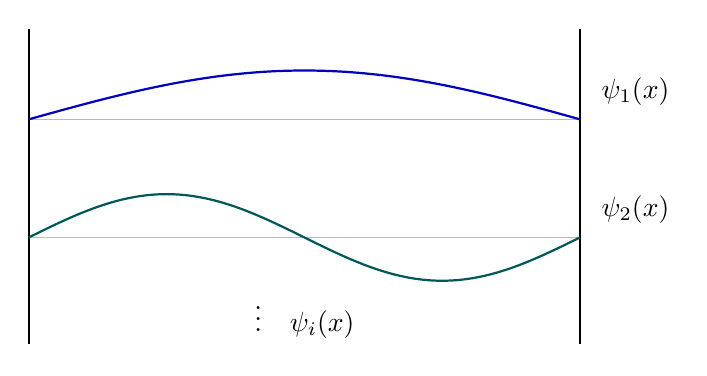
\begin{tikzpicture}[x=1cm,y=1cm]
  \draw[thick] (0,0) -- (0,4.0);
  \draw[thick] (7,0) -- (7,4.0);
  \draw[gray!55] (0,2.85) -- (7,2.85);
  \draw[gray!55] (0,1.35) -- (7,1.35);
  \draw[blue!75!black,thick,domain=0:7,samples=120]
    plot (\x,{2.85+0.62*sin(180*\x/7)});
  \draw[teal!70!black,thick,domain=0:7,samples=120]
    plot (\x,{1.35+0.55*sin(360*\x/7)});
  \node[right] at (7.15,3.20) {$\psi_1(x)$};
  \node[right] at (7.15,1.70) {$\psi_2(x)$};
  \node at (3.5,0.38) {$\vdots\quad\psi_i(x)$};
\end{tikzpicture}
\caption{对定性盒中草图的清晰重建。垂直偏移只是为了显示而将两个波函数分开。}
\end{figure}

正交归一性是
\begin{equation}
\int dx\,\psi_i^*(x)\psi_j(x)=\delta_{ij}.
\label{eq:l07-orthonormality}
\end{equation}
如果\(i=j\)，态是归一化的，积分为一。如果\(i\ne j\)，两个态正交，积分消失。

完备性是同样重要的陈述
\begin{equation}
\sum_i |i\rangle\langle i|=\mathbf 1.
\label{eq:l07-resolution}
\end{equation}
每个\(|i\rangle\langle i|\)投影到一个基方向上；对完备基求和就是恒等算符。作用在任意矢量上只是把该矢量分解为分量再重新组合起来。

现在把方程~\eqref{eq:l07-resolution}夹在两个位置态之间：
\begin{align}
\langle y|x\rangle
&=\sum_i\langle y|i\rangle\langle i|x\rangle \\
&=\sum_i\psi_i(y)\psi_i^*(x) \\
&=\delta(y-x).
\label{eq:l07-position-completeness}
\end{align}
星号属于其左矢-右矢顺序为\(\langle i|x\rangle\)的因子。交换\(x\)和\(y\)给出复共轭但等价的形式。因此，每个完备正交归一基都给出{\proseunicodefont δ}函数的一种表示。正弦、余弦、振子波函数和能量本征函数都起同样的作用。

\begin{classroomqa}
\lecturetimestamp{00:13:43}
\audiencequestion{完备性求和中的第二个波函数应该带复共轭吗？}
\lecturerresponse{是的。按\(\langle y|i\rangle\langle i|x\rangle\)的顺序，因子是\(\psi_i(y)\psi_i^*(x)\)。保持左矢-右矢顺序可见，可以防止星号被猜测或放错位置。}
\end{classroomqa}

这就是我们所需的单粒子数学。现在我们改变态空间。

\section{作为更大状态空间的Fock空间}

对于许多全同粒子，一个方便的基记录每个单粒子模式上占据了多少粒子：
\begin{equation}
|n_1,n_2,n_3,\ldots\rangle.
\label{eq:l07-fock-basis}
\end{equation}
整数\(n_i\)是模式\(i\)的占据数。这个右矢并不是用花哨记号写出的单粒子态。它属于一个更大的Hilbert空间，其中包含零粒子扇区、每一个单粒子态、每一个双粒子态，等等。这个更大的空间称为Fock空间。

为了改变占据数，对每个模式引入一个产生算符和一个湮灭算符，
\begin{equation}
a_i^\dagger,\qquad a_i.
\end{equation}
前者向模式\(i\)添加一个粒子，而后者从中移除一个粒子。在这个阶段，谐振子语言只是一种记账手段：并不一定存在一个真实的弹簧在振荡。谐振子代数恰好给了我们提升和降低占据数所需的机制。

模式数算符是
\begin{equation}
\begin{aligned}
N_i&=a_i^\dagger a_i,\\
N_i|n_1,\ldots,n_i,\ldots\rangle
&=n_i|n_1,\ldots,n_i,\ldots\rangle.
\end{aligned}
\end{equation}
真空是
\begin{equation}
|0\rangle\equiv|0,0,0,\ldots\rangle,
\qquad
a_i|0\rangle=0
\quad\text{for every }i.
\label{eq:l07-vacuum}
\end{equation}
因此，模式\(i\)中的一个单粒子态是
\begin{equation}
|i\rangle=a_i^\dagger|0\rangle.
\label{eq:l07-mode-created}
\end{equation}
同一个符号\(|i\rangle\)现在既可以读作一个单粒子基矢量，也可以读作该矢量嵌入Fock空间的单粒子扇区。这种嵌入是式~\eqref{eq:l07-mode-created}；周围的语境告诉我们正在讨论哪个空间。

\section{将模式打包成场}

定义湮灭场和产生场为
\begin{equation}
\Psi(x)=\sum_i \psi_i(x)a_i,
\qquad
\Psi^\dagger(x)=\sum_i \psi_i^*(x)a_i^\dagger.
\label{eq:l07-field-expansion}
\end{equation}
大写字母很重要。小写函数\(\psi_i(x)\)是复数；大写\(\Psi(x)\)是Fock空间上的算符。在每个空间点\(x\)处，式~\eqref{eq:l07-field-expansion}给出模式算符的一个不同的线性组合。这就是位置算符值函数的含义。

对于自由粒子，模式函数可以是平面波\(e^{ikx}\)。那么式~\eqref{eq:l07-field-expansion}就是一个Fourier展开，只不过其Fourier系数是算符而不是数。旧术语把普通复数称为\(c\)数，把量子算符称为\(q\)数。模式函数是\(c\)数，与一切对易；\(a_i\)和\(a_i^\dagger\)则带有算符特性。

\(\Psi\)和\(\Psi^\dagger\)都不是Hermitian的。它们的伴随互为对方。两个组合
\begin{equation}
\Psi+\Psi^\dagger,
\qquad
i(\Psi^\dagger-\Psi)
\label{eq:l07-hermitian-combinations}
\end{equation}
是Hermitian的，可以表示可观测量。然而就目前而言，场最有用的地方在于它们是局域地产生、湮灭和计数粒子的工具。

\begin{classroomqa}
\lecturetimestamp{00:21:05}
\audiencequestion{一个算符依赖于\(x\)意味着什么？}
\lecturerresponse{这意味着\(x\)的每个值都选出一个不同的算符。空间依赖性存在于普通的模式函数中，而每个由此得到的线性组合都作用在同一个Fock空间上。}
\end{classroomqa}

\section{产生场做什么}

一个定义在当我们问它做什么时才变得有用。从单粒子扇区中的一个位置本征态出发，并插入单位分解：
\begin{align}
|x\rangle
&=\sum_i |i\rangle\langle i|x\rangle \\
&=\sum_i a_i^\dagger|0\rangle\,\psi_i^*(x) \\
&=\Psi^\dagger(x)|0\rangle.
\label{eq:l07-local-creation}
\end{align}
因此，\(a_i^\dagger\)在确定的模式\(i\)中产生一个粒子，而\(\Psi^\dagger(x)\)在\(x\)处产生一个局域化的粒子。在理想化的位置基中，这种局域化是分布式的；物理制备会使用一个窄波包，但代数含义是相同的。

\begin{classroomqa}
\lecturetimestamp{00:24:48}
\audiencequestion{\(\sum_i|i\rangle\langle i|\)是一个投影吗？}
\lecturerresponse{每一项都是到一个基态上的投影。完整的求和就是单位算符本身，称为单位分解。插入它不改变任何态，但会暴露出该态在所选基中的分量。}
\end{classroomqa}

式~\eqref{eq:l07-local-creation}是场的第一个直接的粒子解释。我们不仅仅给一个抽象算符附上了一个空间标签。我们构造出了在那个空间点上产生一个粒子的操作。

\begin{classroomqa}
\lecturetimestamp{00:28:20}
\audiencequestion{位置空间产生场应该标星号还是标剑号？}
\lecturerresponse{算符伴随用剑号。星号表示普通波函数\(\psi_i(x)\)的复共轭；剑号应加在\(a_i^\dagger\)和\(\Psi^\dagger(x)\)上。}
\end{classroomqa}

\begin{classroomqa}
\lecturetimestamp{00:28:36}
\audiencequestion{在模式展开中，产生算符可以移过波函数吗？}
\lecturerresponse{可以。\(\psi_i(x)\)是\(c\)数，所以它们与每个算符都对易。只有在改变诸如\(a_i\)和\(a_j^\dagger\)这样的非对易算符的顺序时才必须小心。}
\end{classroomqa}

\section{从概率密度到粒子密度}

现在让我们来摆弄一下场。第一个自然的表达式是
\begin{equation}
\int dx\,\Psi^\dagger(x)\Psi(x).
\end{equation}
它看起来像单粒子归一化积分，但其中的因子现在是算符。插入模式展开而不改变其顺序：
\begin{align}
\int dx\,\Psi^\dagger(x)\Psi(x)
&=\int dx
\left(\sum_i a_i^\dagger\psi_i^*(x)\right)\\
&\qquad\times\left(\sum_j a_j\psi_j(x)\right) \\
&=\sum_{i,j}a_i^\dagger a_j
\int dx\,\psi_i^*(x)\psi_j(x) \\
&=\sum_{i,j}a_i^\dagger a_j\,\delta_{ij} \\
&=\sum_i a_i^\dagger a_i.
\label{eq:l07-number-derivation}
\end{align}
因此总粒子数算符为
\begin{equation}
N=\sum_i N_i
=\int dx\,\Psi^\dagger(x)\Psi(x).
\label{eq:l07-total-number}
\end{equation}
对于所讨论的态，有限能量的激发在足够高的模式能量处占据数趋于消失，因此尽管可能的模式列表是无限的，这个总数通常是有限的。

被积函数是局域粒子数密度算符：
\begin{equation}
n(x)=\Psi^\dagger(x)\Psi(x).
\label{eq:l07-density}
\end{equation}
严格来说，人们并不在数学点上测量密度。对于一个小区域\(R\)，人们测量的是
\begin{equation}
N_R=\int_R dx\,n(x),
\label{eq:l07-regional-number}
\end{equation}
该区域内的粒子数。像任何量子可观测量一样，\(N_R\)在任意态中不必具有确定值。重复制备可以产生不同的结果。

\begin{classroomqa}
\lecturetimestamp{00:36:27}
\audiencequestion{\(\Psi^\dagger(x)\Psi(x)\)是多粒子概率密度吗？}
\lecturerresponse{它的直接含义是粒子密度。多粒子概率幅一般依赖于所有粒子坐标。局域双线性量在被对该区域积分时，则计数该小区域内的粒子数。}
\end{classroomqa}

\begin{classroomqa}
\lecturetimestamp{00:38:28}
\audiencequestion{算符\(a_i\)和\(a_i^\dagger\)只作用于态矢量，而不作用于单粒子波函数吗？}
\lecturerresponse{是的。它们作用于诸如\(|n_1,n_2,\ldots\rangle\)这样的Fock空间态。乘在它们前面的单粒子模式函数是普通数，并不是这些升降算符所作用的对象。}
\end{classroomqa}

占据数右矢构成一组基，而不是最一般的态。它们可以被叠加，包括同一总粒子数在不同模式间以不同方式分布的叠加。对于像光子这样的中性粒子，人们还可以叠加不同的总粒子数。方程~\eqref{eq:l07-regional-number}中的算符在每一个这样的态中都保持相同的操作意义。

\begin{classroomqa}
\lecturetimestamp{00:40:01}
\audiencequestion{如果把粒子密度除以总粒子数，它是否就变成在\(x\)处找到一个粒子的概率密度？}
\lecturerresponse{在固定\(N\)、大粒子数情形下，\(N_R/N\)是一个相对频率，通常很好地追踪单粒子概率。它并不是把一次测量结果等同于概率的算符恒等式。在独立粒子图像中，测量计数会涨落，典型涨落量级为\(\sqrt N\)，而一次例外的运行即使不太可能，也可能与概率相差很大。}
\end{classroomqa}

\begin{classroomqa}
\lecturetimestamp{00:42:25}
\audiencequestion{在一个电子态与零电子态的叠加中，电荷守恒会怎样？}
\lecturerresponse{那不是用于固定电荷的封闭扇区的那种叠加。人们可以叠加具有相同总电荷的不同分布。光子不携带电荷，因此不同的光子数扇区不会造成这种问题。电子数和正电子数也可以一起改变，而净电荷保持不变。}
\end{classroomqa}

\section{独立粒子的能量}

下一个可观测量是能量。首先限于彼此不相互作用的粒子。在稀薄系统中，这通常是一个很好的近似。原则上，即使光子也会通过高阶过程相互作用，但普通实验室辐射足够稀薄，因此独立粒子描述极好。

令\(\omega_i\)表示模式\(i\)中一个粒子的能量，其中\(\hbar=1\)。一个模式意味着一个单粒子态。总哈密顿量于是为
\begin{equation}
H=\sum_i\omega_i N_i
=\sum_i\omega_i a_i^\dagger a_i.
\label{eq:l07-mode-hamiltonian}
\end{equation}
每个被占据的模式每有一个粒子就贡献一次其单粒子能量。

\begin{classroomqa}
\lecturetimestamp{00:48:16}
\audiencequestion{\(\omega_i\)是位置的函数吗？}
\lecturerresponse{不是。它是与模式\(i\)相关联的能量本征值。函数\(\psi_i(x)\)依赖于位置；\(\omega_i\)依赖于所选的是哪一个能级。}
\end{classroomqa}

值\(\omega_i\)由单粒子定态薛定谔方程确定。定义
\begin{equation}
h=-\frac{\nabla^2}{2m}+V(x).
\label{eq:l07-one-particle-h}
\end{equation}
于是
\begin{equation}
h\psi_i(x)=\omega_i\psi_i(x).
\label{eq:l07-schrodinger-eigenvalue}
\end{equation}
在一维中，动量算符为\(p=-i\partial_x\)，而\(p^2/(2m)\)变为\(-\partial_x^2/(2m)\)。在三维中，三个二阶导数合并为\(-\nabla^2/(2m)\)。

\begin{figure}[htbp]
\centering
\includegraphics[width=0.94\linewidth]{lecture_07_frame_02.png}
\caption{从\(p^2/(2m)+V(x)\)到单粒子薛定谔本征值方程微分形式的板书过程。方程~\eqref{eq:l07-schrodinger-eigenvalue}是其整理后的重构。}
\lectureframe{00:54:10}
\end{figure}

对于任意归一化的单粒子波函数，熟悉的期望值为
\begin{equation}
\langle h\rangle_\psi
=\int dx\,\psi^*(x)h\psi(x).
\label{eq:l07-one-particle-energy-expectation}
\end{equation}
多粒子公式的提示来自将小写波函数替换为算符值场。这还不是证明；它是我们此刻要检验其正确性的猜测：
\begin{equation}
H=\int dx\,\Psi^\dagger(x)h\Psi(x).
\label{eq:l07-field-hamiltonian}
\end{equation}

\section{先写出答案，再证明它}

将方程~\eqref{eq:l07-field-expansion}代入所提出的哈密顿量：
\begin{align}
\int dx\,\Psi^\dagger h\Psi
&=\int dx
\left(\sum_i a_i^\dagger\psi_i^*(x)\right)
h\left(\sum_j a_j\psi_j(x)\right) \\
&=\sum_{i,j}a_i^\dagger a_j
\int dx\,\psi_i^*(x)h\psi_j(x).
\label{eq:l07-h-expanded}
\end{align}
微分算符\(h\)作用于依赖\(x\)的波函数\(\psi_j(x)\)，而不是作用于模式算符\(a_j\)。由薛定谔方程，
\begin{equation}
h\psi_j(x)=\omega_j\psi_j(x).
\end{equation}
因此，
\begin{align}
\int dx\,\Psi^\dagger h\Psi
&=\sum_{i,j}a_i^\dagger a_j\omega_j
\int dx\,\psi_i^*(x)\psi_j(x) \\
&=\sum_{i,j}a_i^\dagger a_j\omega_j\delta_{ij} \\
&=\sum_j\omega_j a_j^\dagger a_j.
\label{eq:l07-h-proof}
\end{align}
这正是方程~\eqref{eq:l07-mode-hamiltonian}。局域场表达式与所有粒子能量之和是同一个算符。

\begin{figure}[htbp]
\centering
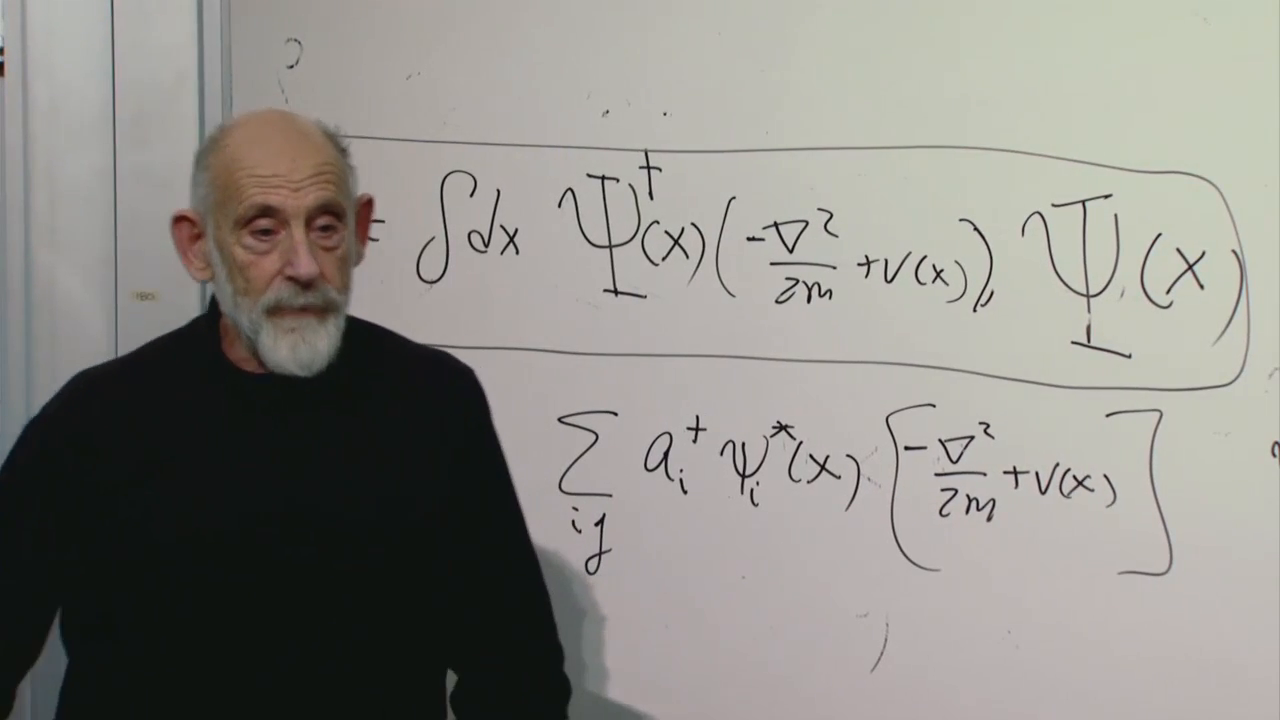
\includegraphics[width=0.94\linewidth]{lecture_07_frame_03.png}
\caption{黑板上强调的场哈密顿量，其下方开始模式展开的证明。保留实时画面作为证据；方程~\eqref{eq:l07-field-hamiltonian}--\eqref{eq:l07-h-proof}恢复了完整的代数运算。}
\lectureframe{01:05:34}
\end{figure}

在此推导中，没有任何产生算符被交换到湮灭算符的另一侧。\(a_i^\dagger a_j\)的顺序自始至终保持不变。唯一可以自由移动的对象是\(c\)数波函数及其本征值。

\section{为什么这是一个场}

为什么称\(\Psi(x)\)为场？因为它是定义在空间每一点上的算符值量，而由它构成的厄米组合或双线性量是局域可观测量。密度\(n(x)\)和下面的局域能量表达式是两个例子。这个词背后并没有隐藏额外的数学检验。

这个场不是电磁场。它描述的是提供单粒子模式和哈密顿量\(p^2/(2m)+V\)的任意非相对论性粒子种类：例如缓慢运动的原子、中子、质子或电子。这些粒子是其对应场的量子，其结构意义与光子是电磁场的量子相同。

\begin{classroomqa}
\lecturetimestamp{01:02:45}
\audiencequestion{在从多粒子系统过渡到上述公式的过程中，场是在哪里进入的？}
\lecturerresponse{它进入于方程~\eqref{eq:l07-field-expansion}：\(\Psi(x)\)在每一个空间点上都是一个算符。随后的推导表明，它的局域乘积度量粒子密度和能量密度。位置依赖性加上算符内容，正是正在构造的场结构。}
\end{classroomqa}

\section{局域能量密度}

方程~\eqref{eq:l07-field-hamiltonian}将总能量写成空间上的积分，
\begin{equation}
\begin{aligned}
H&=\int dx\,\mathcal H(x),\\
\mathcal H(x)
&=-\frac{1}{2m}\Psi^\dagger(x)\nabla^2\Psi(x)\\
&\quad+V(x)\Psi^\dagger(x)\Psi(x).
\end{aligned}
\label{eq:l07-hamiltonian-density}
\end{equation}
被积函数是这个哈密顿量的一个自然的局域能量密度。它的局域形式并不唯一。例如，分部积分将动能项替换为
\begin{equation}
\mathcal H_{\rm kin}(x)
=\frac{1}{2m}\nabla\Psi^\dagger(x)\mathbin{\cdot}\nabla\Psi(x)
\label{eq:l07-kinetic-density}
\end{equation}
相差一个边界项。在通常的边界条件下，两种表达式给出相同的总哈密顿量。这就是讲座中提到的小的模糊性。

\begin{classroomqa}
\lecturetimestamp{01:05:57}
\audiencequestion{能量密度必须在全空间上积分吗？}
\lecturerresponse{在全空间上积分给出总能量。在较小的区域上积分给出分配给该区域的能量，但受制于选择局域密度时通常的模糊性，只要其全积分是同一个哈密顿量。}
\end{classroomqa}

\begin{classroomqa}
\lecturetimestamp{01:06:25}
\audiencequestion{能量公式中的大写\(N_i\)与小写\(n_i\)有何不同？}
\lecturerresponse{\(N_i=a_i^\dagger a_i\)是一个算符。整数\(n_i\)是它在某个粒子数态上的本征值之一。算符作用于态；它们的本征值是普通数。}
\end{classroomqa}

\begin{classroomqa}
\lecturetimestamp{01:06:46}
\audiencequestion{场哈密顿量本身能否用狄拉克符号写成左矢或右矢？}
\lecturerresponse{不能。左矢和右矢表示态矢量及其对偶。场和哈密顿量是作用于这些态的算符。像\(\langle\Phi|H|\Phi\rangle\)这样的期望值同时使用两类对象，绝不能将它们混为一谈。}
\end{classroomqa}

\section{恢复单粒子并接近经典场}

这个扩大的形式体系包含普通的单粒子量子力学。将福克空间限制在满足下式的态上
\begin{equation}
N|\Phi\rangle=|\Phi\rangle.
\end{equation}
在该子空间内，场的构造重现每一个单粒子态和每一个单粒子预言。我们并没有取代旧理论；我们只是把它嵌入到一个也能描述零个、两个或任意多个粒子的空间中。

在另一个极端，被大量玻色子占据的模式可以近似地表现得像经典波。在合适的相干态或半经典态中，期望值
\begin{equation}
\Phi_{\rm cl}(x,t)=\langle\Psi(x,t)\rangle
\end{equation}
对于自由非相对论理论满足一个看似经典的方程
\begin{equation}
i\partial_t\Phi_{\rm cl}(x,t)
=\left(-\frac{\nabla^2}{2m}+V(x)\right)\Phi_{\rm cl}(x,t)
\label{eq:l07-classical-schrodinger}
\end{equation}
讲义陈述了这一联系，而非推导它。它是量子集合与波场之间的桥梁：大占据数抑制相对涨落，并使合适的期望值表现出经典行为。

因此，这一形式体系既是记账，也是物理。它组织所有粒子数扇区，但也刻画干涉、纠缠以及经典波从量子粒子中的涌现。

\begin{classroomqa}
\lecturetimestamp{01:10:43}
\audiencequestion{为什么产生和湮灭算符在积分内部几乎可以像普通数一样被操作？}
\lecturerresponse{它们从未彼此交换过。普通模式函数与它们对易，而导数只作用于那些函数。将一个湮灭算符移过一个产生算符将需要用到对易子，并可能增加一项；证明中没有任何步骤进行这种移动。}
\end{classroomqa}

\section{狄拉克符号插曲}

部分混淆是历史性的。单粒子波函数满足一个波动方程，表面上看起来像经典场，但它同时也是一个概率幅。早期量子理论必须区分这些角色，然后解释诸如电磁学这类真正可测量的波场如何由量子构成。福克空间与算符值场解决了这一表面冲突。

狄拉克符号使这种区分变得异常紧凑。右矢属于一个向量空间，左矢属于其对偶空间，而它们的并置构成内积。完备性关系
\begin{equation}
\sum_i|i\rangle\langle i|=\mathbf 1
\end{equation}
于是几乎不言自明。讲义用一则向数学家教授量子力学的轶事来说明这一点：数学内容早已熟悉，但符号使常规操作如此透明，以至于结构看起来是新的。要点并不是某一学科缺乏这一概念，而是一个选择得当的符号可以使合法操作难以混淆。

这一教训在这里很重要。现在有若干不同的算符：
\begin{itemize}
\item \(h\) 作为微分算符作用于单粒子波函数；
\item \(a_i\) 和 \(a_i^\dagger\) 作用于福克空间中的占据数态；
\item \(\Psi(x)\)、\(\Psi^\dagger(x)\)、\(N\) 和 \(H\) 也作用于福克空间。
\end{itemize}
方程~\eqref{eq:l07-field-expansion}中的展开连接了前两种设定，但没有将它们合并。

\begin{classroomqa}
\lecturetimestamp{01:18:16}
\audiencequestion{场仅仅是一种描述粒子集合的形式体系吗？}
\lecturerresponse{它们是一种形式体系，但并非空洞的形式体系。它们的局域可观测量可以被测量，而粒子是具有干涉和纠缠的量子粒子，而非经典弹丸。场算符恰恰编码了那些可测量的集体性质。}
\end{classroomqa}

\section{相对论性告诫与电磁学旁注}

迄今为止的构造是非相对论性的。在相对论物理中，动量仍然是良好的粒子标签，但尖锐局域化的粒子位置则要微妙得多。因此，局域光子数密度通常不像非相对论性的 \(n(x)\) 那样是一个干净的客体。能量密度仍然定义良好，是更安全的局域可观测量。

讲义给出了一个有用且明确为启发式的电磁类比。将电场和磁场组合成复矢量
\begin{equation}
\mathbf F=\mathbf E+i\mathbf B,
\qquad
\mathbf F^*=\mathbf E-i\mathbf B.
\label{eq:l07-riemann-silberstein}
\end{equation}
于是
\begin{equation}
\mathbf F^*\mathbin{\cdot}\mathbf F
=\mathbf E^2+\mathbf B^2,
\label{eq:l07-em-density}
\end{equation}
在常规单位下正比于电磁能量密度。这字面上并不是光子概率密度。更好的看法是，它是一个紧凑的场变量，其模平方度量能量密度，或者非正式地看作按光子能量加权的光子密度。

\begin{classroomqa}
\lecturetimestamp{01:19:10}
\audiencequestion{光子密度可以与电场强度等同吗？}
\lecturerresponse{只能定性地、并且谨慎地这样说。对于相对论性光子，局域粒子数并非首选概念。稳健的陈述是 \(E^2+B^2\) 正比于能量密度，而复组合 \(\mathbf E+i\mathbf B\) 将麦克斯韦方程打包成类薛定谔形式。}
\end{classroomqa}

\begin{classroomqa}
\lecturetimestamp{01:20:09}
\audiencequestion{为什么相对论性粒子可以有确定的动量，而位置却有问题？}
\lecturerresponse{动量能够干净地标记相对论性单粒子表示，而严格的定域化则与粒子产生及相对论性场描述相冲突。本讲不展开该理论；这一提醒标志着当前非相对论性密度诠释的界限。}
\end{classroomqa}

\section{排序与基态常数}

算符的顺序不能随意改变。对于玻色模式，
\begin{equation}
a_i a_i^\dagger=a_i^\dagger a_i+1.
\end{equation}
因此，将正规序 \(\Psi^\dagger h\Psi\) 替换为反序 \((h\Psi)\Psi^\dagger\)，或其适当积分后的对应形式，会加上对易子贡献。在模式基下，这是每个模式一个能量量子的相加项。它就是基态常数或零点常数，而在连续情形中它需要正规化。本讲在此不追究该问题；只是提醒这两种排序并不相等。

\begin{classroomqa}
\lecturetimestamp{01:22:04}
\audiencequestion{如果在哈密顿量中交换 \(\Psi\) 与 \(\Psi^\dagger\)，会发生什么？}
\lecturerresponse{必须计入它们的对易子。因此，颠倒顺序会加上一个与态无关的基态贡献，而不是重现同一表达式。所展示的哈密顿量保持正规序，\(\Psi^\dagger h\Psi\)。}
\end{classroomqa}

\section{动量作为最终检验}

最后几分钟再次重复了同样的提升。对于单粒子，
\begin{equation}
\langle p\rangle_\psi
=\int dx\,\psi^*(x)\left(-i\partial_x\right)\psi(x).
\label{eq:l07-one-particle-momentum}
\end{equation}
将波函数替换为场，得到总动量算符
\begin{equation}
P=\int dx\,\Psi^\dagger(x)\left(-i\partial_x\right)\Psi(x),
\label{eq:l07-field-momentum}
\end{equation}
或者，在三维中，
\begin{equation}
\mathbf P=\int d^3x\,\Psi^\dagger(\mathbf x)
\left(-i\boldsymbol\nabla\right)\Psi(\mathbf x).
\end{equation}
场携带动量。足够强的激光将动量传递给墙壁并施加力；在量子描述中，该场动量就是光子动量的总和。

式~\eqref{eq:l07-field-momentum} 是算符，而不是期望值。给定一个 Fock 空间态 \(|\Phi\rangle\)，随后可以计算
\begin{equation}
\langle P\rangle_\Phi=\langle\Phi|P|\Phi\rangle.
\end{equation}
要构成期望值，算符和态二者都必不可少。把可观测量与其平均值混为一谈，恰恰会抹去本讲努力建立起来的区分。

\begin{classroomqa}
\lecturetimestamp{01:26:02}
\audiencequestion{所展示的场动量已经是平均动量了吗？}
\lecturerresponse{不是。它是表示该可观测量的厄米算符。给定一个态，并将该算符夹在其左矢与右矢之间，才能得到期望值；测量仍可能围绕该平均值涨落。}
\end{classroomqa}

这是自然的停止点。从粒子出发，我们构造了定域的产生场与湮灭场，用它们来计数粒子，并把单粒子能量与动量之和改写为场算符。下一步不是又一次记号改变，而是让场算符表示物理过程：粒子衰变、粒子散射，以及不同种类相互转化。
